\lstset{language=Java, numbers=left, numberstyle=\tiny, stepnumber=2, numbersep=5pt}
\chapter{Introduction}
\label{intro}
In today's world, where increasingly large amounts of data have to be processed and exchanged by distributed systems, the requirements for communication between distributed systems are becoming more and more complex. Not only performance is a problem, but also the requirement to make the services of the distributed systems available to several users at the same time. In other words, every system that is part of the architecture of a distributed system must be able to communicate with every other subsystem at the same time.\\
There are several technologies in the Java environment that can be used for communication within such a distributed system. The most basic variant is the use of Java Sockets. But this assignment favors the Java Remote Method Invocation. This report considers both technologies and presents a possible solution for a distributed system in which both of them play a role.
%%%%%%%%%%%%%%%%%%%%%%%%%%%%%%%%%%%%%%%%%%%%%%%%%%%%%%%%%%%%%%%%%%%%%%%%%%%%%%%%%%%%%%%%%%%%%%%%%%%%%%%%%
%%%%%%%%%%%%%%%%%%%%%%%%%%%%%%%%%%%%%%%%%%%%%%%%%%%%%%%%%%%%%%%%%%%%%%%%%%%%%%%%%%%%%%%%%%%%%%%%%%%%%%%%%
%%%%%%%%%%%%%%%%%%%%%%%%%%%%%%%%%%%%%%%%%%%%%%%%%%%%%%%%%%%%%%%%%%%%%%%%%%%%%%%%%%%%%%%%%%%%%%%%%%%%%%%%%
\chapter{Network Programming in Java}
\label{network-programming}
This chapter explains the theoretical basis for this assignment. The first section focuses on Java sockets, while the second deals with Remote Method Invocation (RMI). The aim is to highlight the differences as well as the advantages and disadvantages of both technologies.
\section{Sockets in Java}
A socket is an endpoint of a bi-directional communication connection between two programs running in different processes on the same computer or on different computers in a network . One socket takes on the role of the server, while the second socket acts as a client. Socket classes are used in Java to represent the connection between a client program and a server program. Sockets provide a simple API and require a hostname and a free port number to be initialized. If two or more sockets are running on the same computer, the hostnames and portnumbers must be different. Before the two processes (no matter if they are running on different computers or not) can communicate with each other, the client and server sockets must perform two different tasks.
\\
First of all, the client must know the hostname and port number of the server in order to connect to it. How exactly this is done depends on the programmer's decision. The server's address data can be stored permanently in the client's program code or can be retrieved by other techniques such as DNS. When establishing a connection between client and server, the client must also identify itself by sending its own host address to the server. The only thing the server has to do is to listen to possible clients attempting to open a connection.
\\
After the connection has been established, data can be transferred in both directions between server and client. The next two chapters show two different socket types and their differences.
\subsection{TCP Socket}
In general there are two different socket types. The first is the \textbf{Stream Socket} whose communication is based on the Transmission Control Protocol (\textbf{TCP}). Because TCP is connection oriented, the Three-Way-Handshake routine must be performed between server and client. This ensures a stable connection between the two end points via which data can be transmitted. TCP also has a built-in error recovery routine which automatically detects and attempts to fix connection terminations, lost data packets and other failures. The main advantage of this kind of socket is that the communication is safer, because lost packets are detected and resent by the sender (server or client). The main disadvantage is, that these sockets have a larger overhead with the complicated connection establishment and error recovery routines and are therefor slower. Figure \ref{tcpsocket} shows the necessary function calls, both Stream sockets must perform to establish a connection and transmit data:\\
\begin{figure}[H]
	\centering
	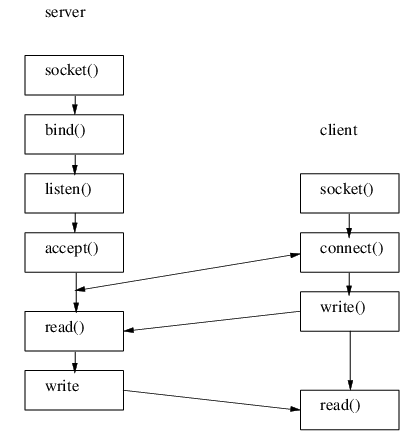
\includegraphics[width =0.7\textwidth]{tcpsocket.PNG}
	\caption{TCP communication between server and client}
	\label{tcpsocket}
\end{figure}
\subsection{UDP Socket}
The \textbf{Datagram Socket} is used for \textbf{UDP} (User Datagram Protocol) communication between two endpoints in the network or between two processes on the same computer.
\\Unlike TCP, UDP does not work connection-oriented. Here the transmitter sends its packets to the destination without worrying about whether the destination is reachable at all. There is also no error recovery because the sender doesn't care if its packets get lost or not. Datagram sockets are only used in certain use cases. Normally, the sender does care whether its packets arrive at their destination or not, which is why this type of communication is rarely used. UDP is only an alternative if the same information is repeated at short intervals, or if the receiver can easily restore missing information using the context. The main advantage however is that UDP is much faster than other network protocols. Figure \ref{udpsocket} shows the function calls both Datagram sockets must perform to transmit data to each other:\\
\begin{figure}[H]
	\centering
	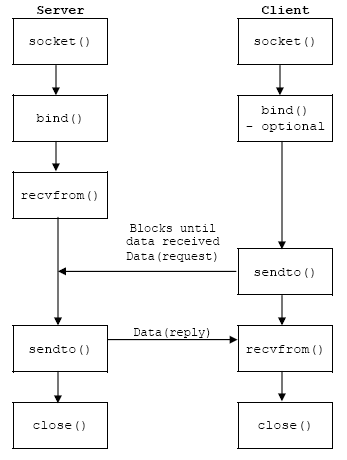
\includegraphics[width =0.6\textwidth]{udpsocket.PNG}
	\caption[Caption for LOF]{UDP communication between server and client\footnotemark}
	\label{udpsocket}
\end{figure}
\footnotetext{image-source: http:///www.tenouk.com//Module41a.html}
\section{Java Remote Method Invocation}
Remote Method Invocation (\textbf{RMI}) enables the call of a method of a remote Java object. The target object is located in another Java virtual machine that can run on a remote or local computer. The call looks exactly like a local call for the calling object, but special exceptions must be caught that can signal connection errors. This technique makes it very easy to build a distributed system in Java, which seems to communicate via normal method calls. For example, RMI can be used to outsource compute-intensive tasks to connected systems that have stronger processors or are simply less busy at the moment. 
\\
Again the basic architecture for RMI is distributed in a client and a server system. The server specifies an interface describing the method or methods that can be called remotely. This interface is called \textit{Remote Interface}. For the client to be able to call a remote method, it must also know this remote interface. The server however must provide a class which implements this interface and therefor provides a real method that can be invoked. This class must also inherit from the \textit{UnicastRemoteObject} class so that the JVM can create stubs and skeletons. The stub is a proxy object, which is required by the client to call the remote method. The skeleton is the proxy of the object on the server side.
\\
Because the remote method offers the possibility to pass parameters and return return values to the caller, some additional information has to be considered. It is possible to pass and return simply data types such as integers or strings without taking further action. But if the user wants to transfer complex objects such class-instances, their classes must implement the \textit{Serializable}-Interface.
\\
Parameters can be transferred via \textit{Object by Value} and \textit{Object by Reference}. The first means that a copy of the object is sent from the client to the server or the other way around. In the case of the second, a real reference to the object is transferred.
\\
The remote object (or service object) must be registered in the RMI registry, which is part of the JRMI environment. This is done with a unique name. This is necessary because the client uses this name to retrieve the object reference from this registry and thus obtains access to the service object. The communication between client and server is based on a simple request/reply protocol. This is why only the client can call methods on the server remotely. The other way around isn't possible. All server-methods that can be called remotely must also throw a \textit{RemoteException} if there is a connection error. Figure \ref{rmi} shows RMI's architecture:
\begin{figure}[H]
	\centering
	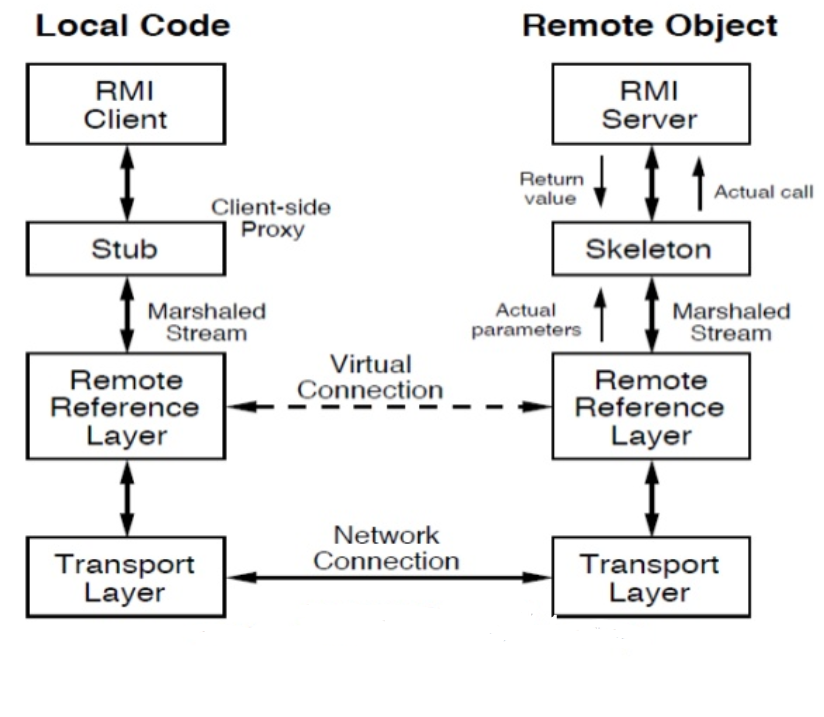
\includegraphics[width =0.8\textwidth]{rmi.png}
	\caption[Caption for LOF]{The RMI architecture\footnotemark}
	\label{rmi}
\end{figure}
\footnotetext{image-source: https://www.slideshare.net/tedionn/java-rmi-26537540}

%%%%%%%%%%%%%%%%%%%%%%%%%%%%%%%%%%%%%%%%%%%%%%%%%%%%%%%%%%%%%%%%%%%%%%%%%%%%%%%%%%%%%%%%%%%%%%%%%%%%%%%%%
%%%%%%%%%%%%%%%%%%%%%%%%%%%%%%%%%%%%%%%%%%%%%%%%%%%%%%%%%%%%%%%%%%%%%%%%%%%%%%%%%%%%%%%%%%%%%%%%%%%%%%%%%
%%%%%%%%%%%%%%%%%%%%%%%%%%%%%%%%%%%%%%%%%%%%%%%%%%%%%%%%%%%%%%%%%%%%%%%%%%%%%%%%%%%%%%%%%%%%%%%%%%%%%%%%%
\chapter{Job Server/Client Architecture}
\label{job}
\section{Overall Architecture}
\section{UDP-Multicast}
\section{The Job Server}
\section{The Job Client}
\section{Workload-Balancing}
%%%%%%%%%%%%%%%%%%%%%%%%%%%%%%%%%%%%%%%%%%%%%%%%%%%%%%%%%%%%%%%%%%%%%%%%%%%%%%%%%%%%%%%%%%%%%%%%%%%%%%%%%
%%%%%%%%%%%%%%%%%%%%%%%%%%%%%%%%%%%%%%%%%%%%%%%%%%%%%%%%%%%%%%%%%%%%%%%%%%%%%%%%%%%%%%%%%%%%%%%%%%%%%%%%%
%%%%%%%%%%%%%%%%%%%%%%%%%%%%%%%%%%%%%%%%%%%%%%%%%%%%%%%%%%%%%%%%%%%%%%%%%%%%%%%%%%%%%%%%%%%%%%%%%%%%%%%%%
\chapter{Other possible solutions}
\label{other-solutions}
\section{Server Broadcast}
\section{Workload Balancer}

%%%%%%%%%%%%%%%%%%%%%%%%%%%%%%%%%%%%%%%%%%%%%%%%%%%%%%%%%%%%%%%%%%%%%%%%%%%%%%%%%%%%%%%%%%%%%%%%%%%%%%%%%
%%%%%%%%%%%%%%%%%%%%%%%%%%%%%%%%%%%%%%%%%%%%%%%%%%%%%%%%%%%%%%%%%%%%%%%%%%%%%%%%%%%%%%%%%%%%%%%%%%%%%%%%%
%%%%%%%%%%%%%%%%%%%%%%%%%%%%%%%%%%%%%%%%%%%%%%%%%%%%%%%%%%%%%%%%%%%%%%%%%%%%%%%%%%%%%%%%%%%%%%%%%%%%%%%%%
\chapter{Conclusion}
\label{conclusion}
